\documentclass[preprint]{aastex}

% packages for figures
\usepackage{graphicx}
% packages for symbols
\usepackage{latexsym,amssymb,hyperref}
% AMS-LaTeX package for e.g. subequations
\usepackage{amsmath}


\usepackage[OT2,T1]{fontenc}


%=====================================================================
% FRONT MATTER
%=====================================================================

\slugcomment{Draft \today}

%=====================================================================
% BEGIN DOCUMENT
%=====================================================================

\newcommand{\kmax}{\ensuremath{k_\mathrm{max}}}
\newcommand{\kmin}{\ensuremath{k_\mathrm{min}}}
\newcommand{\rmd}{\ensuremath{\mathrm{d}}}
\newcommand{\beq}{\begin{equation}}
\newcommand{\eeq}{\end{equation}}
\newcommand{\mi}{{\rm i}}
\newcommand{\me}{{\rm e}}

\DeclareSymbolFont{cyrletters}{OT2}{wncyr}{m}{n}
\DeclareMathSymbol{\Sha}{\mathalpha}{cyrletters}{"58}

\begin{document}

\title{Lensing engine testing and normalization convention (Issue \#248)}

\begin{abstract}
This document contains Rachel's notes on tests of the lensing engine
for GalSim Issue \#248.  There are a number of questions we need to
check to make sure that that software is doing what we want it to do,
and all the relevant tests and equations are described below.
\end{abstract}

\section{Introduction}

There are a few issues that we wish to check regarding the lensing
engine.  They are:

\begin{enumerate}
\item Overall normalization of shear variance: Currently the shear
  variance for a constant input shear power does not depend on
  the grid size/shape.  This seems non-standard, so we should
  investigate and understand this further.
\item We need to check the scaling of either the observed correlation
  function or power spectrum with $k$, to make sure it is done right.
\item What is the effect of interpolating between grid points?  does
  the interpolant have the expected impact on the shear power?
\item If we put in just $E$ or just $B$ mode power with a flat
  spectrum, the variances of $\gamma_1^2$ and $\gamma_2^2$ differ; is
  this expected for a flat power spectrum or sign of a problem?
\item We should make sure that when we use both $E$ and $B$ mode
  power, that we get the expected result, and that results with only
  $E$ or only $B$ are also sane.
\item Impact of differences between continuous vs. discrete
  representation?
\end{enumerate}

\textbf{Important update: In tracing through the code, I realized that
  the dimensions were not being handled properly. We were taking the
  square root of the power, which gives a quantity that has dimensions
  of angle, and then using that to generate shears.  I propose a
  division by grid spacing at that step, to get a dimensionless
  quantity.  Given the size of the grid spacing, this can
  change results by orders of magnitude!  Results below are discussed both without and with that fix.}

\section{Theory}\label{sect:theory}

The lensing engine requires a shear power spectrum, $P(k)$.  We are
working in the flat-sky limit, so when we see expressions in terms of
$\ell$ we can swap $\ell$ with $k$ and $C_\ell$ with $P$, and
\beq
\Delta^2 = \frac{\ell(\ell+1) C_{\ell}}{2\pi}\equiv \frac{k^2 P(k)}{2\pi}.
\eeq
When people plot shear power spectra they usually actually plot
$\Delta^2(k)$ (or, in terms of the full-sky formalism, they plot $\ell(\ell+1)C_\ell/(2\pi)$).

If we identify pairs of galaxies and get the shears in a coordinate
system defined along the vector connecting them ($\gamma_+$) and at 45
degrees with respect to it ($\gamma_\times$), then we can compute
correlation functions of the $\gamma_+$ and $\gamma_\times$ values,
which we will call $\xi_{++}$ and $\xi_{\times\times}$.  Then the
standard cosmological correlation functions $\xi_{\pm}$ are defined as
\begin{align}
\xi_{\pm}(\theta) &=  \xi_{++}\pm \xi_{xx} \\
 &= \frac{1}{2\pi}\int k\,\rmd k P(k) J_{0/4}(k\theta).  \label{eq:xi}
\end{align}

Since correlation functions are dimensionless, we immediately see that
$P(k)$ has dimensions of angle$^2$ and $\Delta^2(k)$ is dimensionless.

The variance of the shear values, 
\beq
\mathrm{Var}(\gamma) = \langle g_1^2 + g_2^2\rangle,
\eeq
is essentially $\xi_+(\theta=0)$.   Note that this is what we get for
the defined $\xi_+$ in the limit of $\theta$ going to zero, but that
equation was defined in terms of $\gamma_+$ and $\gamma_\times$ rather
than $\gamma_1$ and $\gamma_2$.  On a grid, it's not clear that we
can enforce/check behavior of Var($\gamma_1$) or Var($\gamma_2)$,
particularly if the corners are important (which will be the case if
there is a lot of shear power at small $k$), probably we should 
 only expect normal behavior for Var($\gamma$), but it's still worth
 verifying this.  So, combining several equations,
\beq\label{E:shearvar}
\mathrm{Var}(\gamma) = \frac{1}{2\pi}\int k\,\rmd k P(k).
\eeq
which essentially says the shear variance is the power integrated over
the allowed area in $k$ space.  I {\em think} (Barney: \emph{you are
  right I am almost certain, see Section \ref{sect:DFTPS}}) that if we want to work
in terms of $k_x$ and $k_y$, we can replace $2\pi k\rmd k$
(integrating within a circle) with $\rmd
k_x \rmd k_y$ (integrating within our square grid), so the above might also be
written as
\beq\label{E:alt-shearvar}
\mathrm{Var}(\gamma) = \frac{1}{(2\pi)^2} \int \rmd k_x \rmd k_y
P(k_x, k_y).
\eeq

None of these integrals have had limits on them.  Formally they should
go from the minimum to the maximum accessible $k$ on our grid.  Our
grid is defined by
\begin{align}
L &= \mbox{length of grid along one dimension (angular units)}\\
d &= \mbox{spacing between grid points (angular units)}\\
N &= \mbox{number of grid points along one dimension} = L/d
\end{align}

In all of the above I have simply written $P(k)$ but in principle there can be
two such functions, $P_{E}$ and $P_B$.  I believe these
should simply be summed in the above variance equation, but should check this.

A note about something possibly confusing: there are many papers that
write equations for shear variances that include some window function,
which we haven't included here.  I believe that is okay, because those
papers are referring to a different calculation: they are averaging
the shear in some cells, and computing the expected variance of those
shears that have been averaged in cells.  In contrast, we're computing
the variance of individual shears that have been defined within our
grid, which is a completely different thing.

\section{Comparison software}

We will compare against a completely independent piece of software,
Chris Hirata's spherical harmonic transform code which is described in
multiple papers (for example,
\href{http://adsabs.harvard.edu/abs/2004PhRvD..70j3501H}{Hirata
  et~al. 2004}).  This does not use the flat-sky
approach, but that should not be huge important of a difference even
for our $L=10$ deg.  It is something to bear in mind if we start
looking for agreement at a few \% level on the largest $\theta$ or
smallest $k$.  This software wants $C_\ell(\ell)$ as its inputs.

\section{General considerations for these tests}

First, it's not clear that we should really be enforcing $P(0)=0$,
i.e., no power below our \kmin.
This is a valid condition for the full-sky power spectrum, but will
not in general be valid for a small patch of the sky, due to sampling
variance.  In order to include this sampling variance, it would be
preferable to assign $P(0)=$ some kind of integral over $P(k<\kmin)$
(perhaps an average power in that $k$ range; details to be worked out later) assuming the power function is
defined for those value of $k$.

Second, since we use a DFT of a finite set of samples, we implicitly
have a $k$ defined on a periodic grid, not simply $P(k)=0$ for all
$k>\kmax$.  This also means that we should possibly avoid using the
variance as a metric, because what we really care about is whether the
PS is represented properly within our $k$ range.

Moreover, we need to be well-sampled in $k$ space, so we should not
use functions that do unreasonable things like $k^{-2}$.

\subsection{Variance for Gaussian $P(k)$}

Barney suggested a test case that is a Gaussian, i.e., $P(k) =
P_0 e^{-\sigma^2 k^2 / 2}$.  Here both $P_0$ and $\sigma^2$ both
are dimensions of angle$^2$.  By my calculations, this means that
\begin{align}
\mathrm{Var}(\gamma) &= \frac{P_0}{2\pi}\int_{\kmin}^{\kmax} k \,
e^{-\sigma^2 k^2/2} \,\rmd k \\
 &= \frac{P_0}{2\pi\sigma^2} (e^{-\kmin^2\sigma^2/2}-e^{-\kmax^2\sigma^2/2}).
\end{align}

We use three grids. The first is the standard GREAT10 grid with $L=10$
degrees and $N=100$, so $d=0.1$ deg $=360$ arcsec.  I will define the
Gaussian such that there is essentially no power left at our \kmax,
which is $2\pi/d=0.0175$ arcsec$^{-1}$.  the second grid has the same
$d$ but only 50 grid points per dimension, so it covers $5$ degrees.
Using this grid lets us test for sensitivity to \kmin\ at fixed \kmax.
The third grid covers the original $L=10$ deg, but with $N=50$, so
$d=0.2$ deg $=720$ arcsec; this grid (compared to the first one) has the same \kmin\ and different \kmax. We use $\sigma \kmax=5$ or $\sigma=286.5$
arcsec for the first two grids; we want to keep the same condition on
$\sigma\kmax$ for the last grid, so in that case we use
$\sigma=573.0$.  In all cases, $\sigma\kmin$ is quite close to zero,
so the variance we expect should be quite close to
$P_0/(2\pi\sigma^2)$. We will set $P_0=1$. The code is:
\begin{verbatim}
import galsim
import numpy as np
test_ps = galsim.PowerSpectrum(lambda k : np.exp(-0.5*((286.5*k)**2)))
g1, g2 = test_ps.buildGriddedShears(grid_spacing=360., ngrid=100)
print np.var(g1), np.var(g2), np.var(g1)+np.var(g2)
g1, g2 = test_ps.buildGriddedShears(grid_spacing=360., ngrid=50)
print np.var(g1), np.var(g2), np.var(g1)+np.var(g2)
test_ps = galsim.PowerSpectrum(lambda k : np.exp(-0.5*((573.0*k)**2)))
g1, g2 = test_ps.buildGriddedShears(grid_spacing=720., ngrid=50)
print np.var(g1), np.var(g2), np.var(g1)+np.var(g2)
\end{verbatim}

The results are around $1.8\times 10^{-6}$ in the first two cases, and
$4.6\times 10^{-7}$ in the last case.  Our expectations are around
$3\times 10^{-7}$ for the first two cases, and $7.7\times 10^{-8}$.
So the scaling with the grid spacing and grid size is okay, but the
amplitude is off by a factor of $\sim 6$. Need to investigate whether
this could be due to a missing factor of $2\pi$ in my prediction of
the variance. \textbf{These results are with the version of GalSim
  with the dimensionality fix.  Before that, the variances were all
  the same, which means the scaling with $\sigma$ was wrong.}

Note that the variance is evenly divided into the two components.

\subsection{Variance for flat $P(k)$}

This test is dangerous because of the amount of large-scale power, but
let's check the results anyway.  If we say $P(k)=P_0$, then we expect
\beq
\mathrm{Var}(\gamma) = \frac{P_0}{(2\pi)^2} \times (\kmax-\kmin)^2
\sim \frac{P_0 \kmax^2}{(2\pi)^2}.
\eeq

If I use $P_0=0.01$, and do 
\begin{verbatim}
import galsim
import numpy as np
test_ps = galsim.PowerSpectrum(lambda k : 0.01+np.zeros_like(k))
g1, g2 = test_ps.buildGriddedShears(grid_spacing=360., ngrid=100)
print np.var(g1), np.var(g2), np.var(g1)+np.var(g2)
g1, g2 = test_ps.buildGriddedShears(grid_spacing=360., ngrid=50)
print np.var(g1), np.var(g2), np.var(g1)+np.var(g2)
g1, g2 = test_ps.buildGriddedShears(grid_spacing=720., ngrid=50)
print np.var(g1), np.var(g2), np.var(g1)+np.var(g2)
\end{verbatim}
with the \textbf{updated} version of the lensing engine, then the variances are $\sim 7.7\times 10^{-8}$ (first two cases) and
$1.9\times 10^{-8}$ (last case).  I was expecting, for the first two
cases, a variance of $0.01 (0.0175/2\pi)^2=7.8\times 10^{-8}$, and for
the last case, something that is four times smaller, which is exactly
what I find.  So the variance test seems to work here.  \textbf{Note
  that this did not work out right before the dimensionality issue was
  fixed by dividing by grid spacing!  In that case, the power was
  constant in all cases.}

The variance is not quite divided evenly between components, but that
might be okay; this calculation emphasizes large-scale power, and it's
exactly on scales comparable to the grid size that we expect
differences between $\gamma_1$ and $\gamma_2$ behavior.  In the
previous test, the variance was evenly divided, so that supports this
explanation and suggests we shouldn't worry about this uneven split
for flat $P(k)$.

\section{Test of $P(k)$}\label{S:testpk}

I have a WMAP7 LCDM prediction for the cosmic shear signal for a
sample with $z_{med}\sim 0.55$, which I can use as an input to both
the SHT code and ours.  Given the range of $\ell$ for which it is
defined, $2<\ell<2000$, we cannot use our standard grid because that
has $\kmax=3600$ radians$^{-1}$.  So, for this test I use a grid with
the same $L$ as before, but $N=50$ (i.e., $d$ gets doubled), which
means $\kmax=1800$ radians$^{-1}$.

Using the SHT code, I made gridded shears for each of 3 cases:
$P_E=P(k)$ and $P_B=0$; $P_B=P(k)$ and $P_E=0$; and $P_E=P_B=P(k)$ (5
realizations of each).
For GalSim, since it's less computationally expensive I averaged over
more realizations; for our code, it is crucial to inform the code that
the inputs have units of radians.

The python script test\_pk.py in devel/external/test\_gridshear/ does the following:
\begin{enumerate}
\item Generates shears according to this PS using GalSim.
\item Runs the GREAT10 power spectrum code on both (must flip sign of
  one shear component before doing so), and averages it over several
  noise realizations.
\end{enumerate}

The python script test\_pk\_sht.py in that directory does the following:
\begin{enumerate}
\item Manipulate outputs of the SHT code to be consistent with
  expectations (incl. one sign flip for e1).
\item Runs the GREAT10 power spectrum code on it.
\end{enumerate}

Finally, plot\_pk\_test.py in that directory plots the original and
simulated $P(k)$ based on these files.  The results for the three
cases (input $P_E$, input $P_B$, and input $P_E=P_B$) are in
Figures~\ref{F:pe}, \ref{F:pb}, \ref{F:peb}.  \textbf{These plots have
  all been updated to use the version of the lensing engine with the
  dimensionality fix mentioned in the intro to these notes.}

\begin{figure}
\begin{center}
\includegraphics[width=3in]{../external/test_gridshear/output/compare_input_pe.eps}
\caption{Output shear power spectra (plotted as the dimensionless
  $\Delta^2$) for the grids described in Sec.~\ref{S:testpk}, where
  the input $P_E$ is a realistic cosmological one (shown as the 'theory' line on
  the plot) and the input $P_B=0$. The results for GalSim and the
  comparison SHT code are both plotted.\label{F:pe}}
\end{center}
\end{figure}

\begin{figure}
\begin{center}
\includegraphics[width=3in]{../external/test_gridshear/output/compare_input_pb.eps}
\caption{Output shear power spectra (plotted as the dimensionless
  $\Delta^2$) for the grids described in Sec.~\ref{S:testpk}, where
  the input $P_B$ is a theoretical one and the input $P_E=0$. The results for GalSim and the
  comparison SHT code are both plotted.\label{F:pb}}
\end{center}
\end{figure}

\begin{figure}
\begin{center}
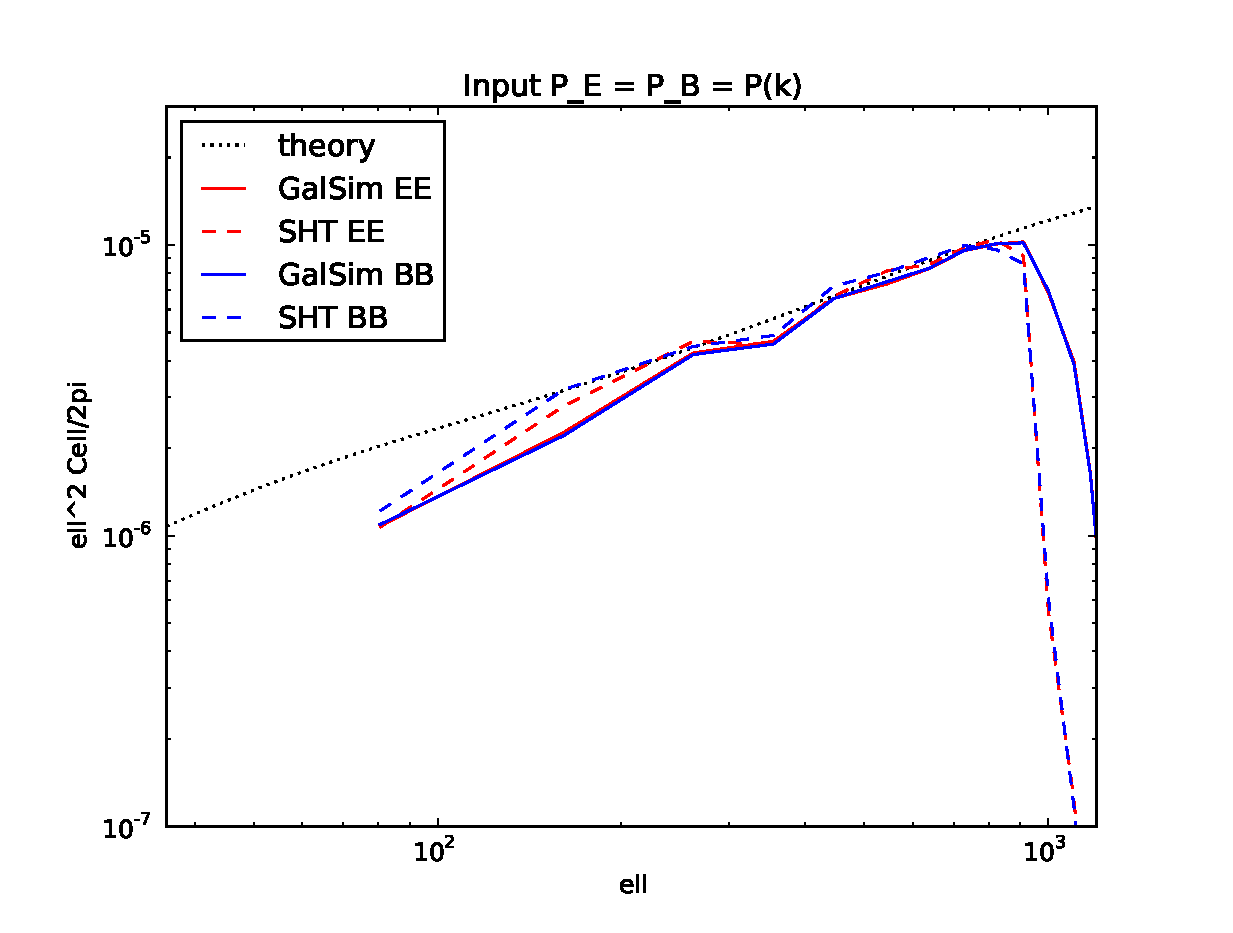
\includegraphics[width=3in]{../external/test_gridshear/output/compare_input_peb.eps}
\caption{Output shear power spectra (plotted as the dimensionless
  $\Delta^2$) for the grids described in Sec.~\ref{S:testpk}, where
  the input $P_E=P_B$ is shown as the 'theory' line. The results for GalSim and the
  comparison SHT code are both plotted.\label{F:peb}}
\end{center}
\end{figure}

Conclusions:
\begin{itemize}
\item \textbf{The dimensionality fix, dividing by grid spacing, has
    gotten rid of nearly all discrepancies between theoretical and
    generated power spectra.}
\item SHT code: it gives roughly a consistent power spectrum compared
  to our inputs (modulo possible slight differences in scaling that
  may not be worth investigating until our own PS code is ready),
  though there are signs of $E$ vs. $B$ leakage in the case where one
  or the other is zero.
\item GalSim: we don't see $E$ vs. $B$ leakage at any significant
  level.  The amplitudes and scaling with $\ell$ are approximately
  correct.
\item While the big-picture results seem good, there are some finer
  details that require investigation, in particular the fact that both
  codes seem to give steeper $P(k)$ than the theory.  Given how these
  tests were done, it could have to do with the $k$-space binning in
  the power spectrum estimator.  I'm not sure how much detail we want
  to dig into here, vs. waiting for our own power spectrum estimator.
\end{itemize}



\section{Representing continuous fields using the Discrete Fourier Transform}

Here is what Barney has managed to learn about this issue, and how we
are numerically representing $P(k)$, in the course of many pages of
handwritten derivation (much of which is of course now scribbled out).

\subsection{Conventions}

The definition of the correlation function in equation \eqref{eq:xi}
employs the \emph{angular frequency, non-unitary}\footnote{According
  to the paradigm setup in
  http://en.wikipedia.org/wiki/Fourier\_transform\#Other\_conventions}
definition of the (1D) Fourier transform:
\begin{eqnarray}
\tilde{f}(k) & = & \int_{-\infty}^{\infty} f(x) \me^{-\mi k x}
dx ~ ~ \equiv ~ \mathcal{F} \{ f(x) \} \label{eq:fwdft} ; \\
f(x) & = & \frac{1}{2 \pi} \int_{-\infty}^{\infty} \tilde{f}(k) \me^{\mi k x}
dk ~ ~ \equiv ~ \mathcal{F}^{-1}\{ \tilde{f}(k) \} \label{eq:invft}, 
\end{eqnarray}
with the usual simple generalizations to two or more dimensions.

The standard results in Discrete Fourier Transform (DFT) and its
halfway-house the Discrete Time Fourier Transform (DTFT) are all
derived under the unitary (i.e. symmetric with no odd factors of $2
\pi$ around) convention in the online literature, adding to the complexity of
interpretation.  This led me to re-derive some standard results of
Fourier theory using the conventions above, which it now makes sense
to state as we will require them in Section \ref{sect:DFTPS}.

\subsection{Fourier transform properties}
It can be readily shown that if we define $g(x L) \equiv f(x)$ the following well-known identity holds
under our Fourier transform convention:
\begin{equation}
\mathcal{F}\{g(x L)\} = \frac{1}{L}
\tilde{g}\left(\frac{k}{L}\right). \label{eq:gmult}
\end{equation}
If we further define $s(h + x) \equiv g(x)$ then it is straightforward
to show that
\begin{equation}
\mathcal{F}\{ s(h + x) \} = \me^{\mi k h} \tilde{s}(k).  \label{eq:sadd}
\end{equation}
Here we begin to get divergent results between conventions: there is
an additional factor of $2\pi$ in the exponent for the normal frequency
convention version of this property.

The most important result for approximating continuous functions using
DFTs is the Poisson summation formula, which under our conventions may
be stated as
\begin{equation}
\sum_{n=-\infty}^{\infty} f(n) = \sum_{q=-\infty}^{\infty} \tilde{f}(2
\pi q)
\end{equation}
for integers $n$ and $q$.  This result can be derived by writing the
  expression for the inverse Fourier transform of $\tilde{f}(2 \pi
q)$ and considering the Fourier series expansion of the periodic Dirac comb
function
\begin{equation}
\Sha_L (x) = \sum_{n=-\infty}^{\infty} \delta(x - nL).
\end{equation}
It should be noted that in the normal frequency, unitary transform
convention form of the Poisson summation formula the $2\pi$ within $\tilde{f}(2 \pi
q)$ is absent.\footnote{Barney would heartily welcome \emph{anyone} wishing to
check his derivations of these results using the non-symmetric
convention!}  Using equation \eqref{eq:gmult} we then find
\begin{equation}
\sum_{n=-\infty}^{\infty} f(n L) = \frac{1}{L}
\sum_{q=-\infty}^{\infty} \tilde{f} \left(\frac{2 \pi q}{L} \right),
\end{equation}
which can be modified further using equation \eqref{eq:sadd} to give
the most useful expression of the Poisson summation formula:
\begin{equation}
\sum_{n=-\infty}^{\infty} f(n L + x) = \frac{1}{L}
\sum_{q=-\infty}^{\infty} \tilde{f} \left(\frac{2 \pi  q}{L} \right)
\me^{\mi 2 \pi x q / L}.
\end{equation}
If we define $\Delta k \equiv k_{\rm min} = 2 \pi / L$ we can also write
this as
\begin{equation}
\sum_{n=-\infty}^{\infty} f\left(\frac{2\pi n}{\Delta k} + x \right) = 
\left(\frac{\Delta k}{2 \pi} \right)
\sum_{q=-\infty}^{\infty} \tilde{f} \left(q \Delta k \right)
\me^{\mi x \Delta k q }. \label{eq:poisson}
\end{equation}
These results give us most of what we need to understand DFTs with the
non-standard Fourier transform convention commonly adopted for weak
lensing power spectra in the flat sky approximation.

\subsection{The Fourier transform of discrete samples of the power spectra}\label{sect:DFTPS}
In what follows we are going to derive results only for the $\xi_+$
correlation function of equation \eqref{eq:xi}.  This will not
not impact upon the understanding of how $P(k)$ is approximated using DFTs,
but allows us to replace $\xi_{\pm}$ and $J_{0/4}(k \theta) $in
equation \eqref{eq:xi} with $\xi$ and $J_0$, respectively.  We will
just be aware subsquently that real ellipticity fields have two
components, to be treated as described by equation \eqref{eq:xi}.

The inverse Fourier transform of $P(k)$ to give $\xi_+(\theta)$ may 
be written in Cartesian coordinates as
\begin{equation}
\xi_{+}(\theta_1, \theta_2)  = \frac{1}{(2 \pi)^2} \int \! \! \!
\int_{-\infty}^{\infty} P(k_1, k_2) ~ \me^{\mi (k_1 \theta_1 + k_2
  \theta_2)} dk_1 dk_2. \label{eq:xip}
\end{equation}
The relation between this and equation \eqref{eq:xi} makes use of Bessel's first
integral:
\begin{equation}
J_n(z) = \frac{\mi^{-n}}{\pi} \int_0^{\pi} \me^{\mi z \cos{\theta}}
\cos{(n \theta)} d \theta,  
\end{equation}
(\emph{which I believes shows you have the correct expression for the
  variance on page 2, Rachel...}).

What happens if we only have finite samples of $P(k_1, k_2)$?  To
answer that, let us define the following function:
\begin{equation}
P_{\Delta k} [q, p] \equiv (\Delta k)^2 P(q \Delta k, p \Delta k).
\end{equation}
As here, we will use square brackets to denote functions with discrete input
variables throughout what follows.  We will also use indices $n, m$ in
real space summations and $q, p$ in Fourier space ($i,j$ are awkward
due to the common notations for $\sqrt{-1}$).  Let us also define the 2D Dirac
comb function in Fourier space
\begin{equation}
\Sha^2_{\Delta k} (k_1, k_2) = \sum_{q = -\infty}^{\infty} \delta(k_1
- q \Delta k) \sum_{p = -\infty}^{\infty} \delta(k_2
- p \Delta k).
\end{equation}
It can then be shown that
\begin{eqnarray}
\mathcal{F}^{-1} \left\{ P_{\Delta k} [q, p] \cdot  \Sha^2_{\Delta k} (k_1,
  k_2) \right\} & = & \mathcal{F}^{-1} \left\{ P(k_1, k_2) \cdot  (\Delta
  k)^2 \Sha^2_{\Delta k} (k_1,
  k_2) \right\}  \nonumber  \\
 & = & \mathcal{F}^{-1} \left\{ P(k_1, k_2) \right\} * \mathcal{F}^{-1} \left\{  (\Delta
  k)^2 \Sha^2_{\Delta k} (k_1, k_2) \right\} \nonumber \\
 & = & \xi_+(\theta_1, \theta_2 )  * \left\{ \sum_{n = -\infty}^{\infty} \delta\left(\theta_1
- \frac{2 \pi n}{\Delta k} \right) \sum_{m = -\infty}^{\infty}
\delta\left( \theta_2
- \frac{2 \pi m}{\Delta k} \right)  \right\} \nonumber \\
& = & = \sum_{n,m=-\infty}^{\infty} \xi_+\left(\theta_1
- \frac{2 \pi n}{\Delta k},  \theta_2
- \frac{2 \pi m}{\Delta k} \right) \label{eq:xisum}
\end{eqnarray}
Here we have again made use of the Fourier series expression for the
Dirac comb function, and employed the convolution theorem (convolution
denoted with $*$).  We note that the final expression \eqref{eq:xisum}
is still continuous, but describes an infinite, periodic summation (of period $L = 2 \pi
/ \Delta k$) of copies of the correlation function $\xi_+$.  For sufficiently small
$\Delta k$, these copies may be well-enough spaced in the real domain to
learn much about $\xi_+(\theta_1, \theta_2)$ in the non-overlapping
regions.

We therefore define this function as
\begin{equation}
\xi_{\frac{2\pi}{\Delta k}}(\theta_1, \theta_2) \equiv \sum_{n = -\infty}^{\infty} \xi_+\left(\theta_1
- \frac{2 \pi n}{\Delta k},  \theta_2
- \frac{2 \pi m}{\Delta k} \right).
\end{equation}
Using the expression of the Poisson summation formula in equation
\eqref{eq:poisson}, we can also write the result
\begin{equation}
\xi_{\frac{2\pi}{\Delta k}}(\theta_1, \theta_2) =
\sum_{q,p=-\infty}^{\infty} \left( \frac{\Delta k}{2 \pi} \right)^2 P(q \Delta k, p \Delta k) \me^{\mi \Delta
  k (\theta_1 q + \theta_2 p)} = \frac{1}{( 2 \pi)^2}
\sum_{q,p=-\infty}^{\infty} P_{\Delta k} [q, p] \me^{\mi \Delta
  k (\theta_1 q + \theta_2 p)}. \label{eq:dtft}
\end{equation}
This is the expression for the inverse of what is known as the
Discrete Time Fourier Transform (DTFT), although this result is
normally derived using unitary conventions for the transform pair.
Note that the terms $P_{\Delta k}[q, p]$ are dimensionless, being
composed of $(\Delta k)^2 = (2 \pi / L)^2$ multiplied by the samples $P(q \Delta k, p \Delta
k)$ of the power $P(k_1, k_2)$ (dimensions angle$^2$).  

One intuitive way of looking at the approximation of equation \eqref{eq:xip} for the case of discretely
sampled $P(k_1, k_2)$ is that the terms in the discrete sum should be
considered as \emph{impulses} of area $(\Delta k)^2$ and height $P(q \Delta k, p \Delta k)$.

\subsection{The Fourier transform of discrete, finite samples of the power spectra}
The expression in equation \eqref{eq:dtft} is periodic with period $2
\pi / \Delta k = L$.  All of the information it contains about
$\xi(\theta_1, \theta_2)$ is therefore also contained in one period
of the functoin only.  For approximating this information discretely, as desired in
numerical analysis, we can imagine taking $N$ equally spaced samples of
the function in equation \eqref{eq:dtft} along a single period $L$ in each
dimension (leading to $N^2$ samples total since we are working in 2D).
These samples are therefore separated by $\Delta \theta \equiv 2 \pi /
\Delta k N = d$ in real space, and we define the sampled
function itself as
\begin{equation}
\xi_{\Delta \theta}[n, m] \equiv \xi_{\frac{2 \pi}{\Delta
    k}} \left( n \Delta \theta, m \Delta \theta \right) = \frac{1}{( 2 \pi)^2}
\sum_{q,p=-\infty}^{\infty} P_{\Delta k} [q, p] \me^{\mi 2 \pi (qn +
  pm) / N}
\end{equation}
for the integer indices $n, m = 0, 1, \ldots, N-1$, substituting into equation
\eqref{eq:dtft}.  Using the periodicity of the exponential term in the
expression above, this may be written as
\begin{equation}
\xi_{\Delta \theta}[n, m] = \frac{1}{( 2 \pi)^2}
\sum_{q,p=0}^{N-1} P_N [q, p] \me^{\mi 2 \pi (qn +
  pm) / N}
\end{equation}
where we have defined
\begin{equation}
P_N[q, p] \equiv \sum_{i,j=-\infty}^{\infty}  P_{\Delta k} [q - i N, p
- j N] .
\end{equation}
Needless to say, in order to be able to calculate the values of
$P_N[q, p]$ in practice we must also truncate the 
$P_{\Delta k}$ sequence to be finite in length.  A \emph{very} common
choice is to use the same number $N$ of samples in both real and
Fourier space: this is also efficient, as it allows the direct use of
the Fast Fourier Transform algorithm.  We will say a little more about
this below.

Choosing to use only $N$
samples from $P_{\Delta k}$ then gives us a more
familiar expression for the inverse Discrete Fourier Transform (DFT),
albeit for the non-unitary Fourier transform convention:
\begin{equation}
\xi_{\Delta \theta}[n, m] = \frac{1}{( 2 \pi)^2}
\sum_{q,p=0}^{N-1} P_{\Delta k} [q, p] \me^{\mi 2 \pi (qn +
  pm) / N}. \label{eq:dft}
\end{equation}
The overwhelmingly more common definition of the inverse DFT, and that adopted by
NumPy, instead reads as:
\begin{equation}
f[n, m] = \texttt{numpy.fft.ifft2}\left(\tilde{f}[p, q]\right) = \frac{1}{N^2}
\sum_{q,p=0}^{N-1} \tilde{f}[q, p] \me^{\mi 2 \pi (qn +
  pm) / N} ,~~~~ (\textrm{NumPy convention}) \label{eq:dftnumpy}
\end{equation}
where the factor of $1/N^2$ is a convention commonly with DFT
implementations, and ensures
that the DFT followed by the inverse DFT yields the original, input array.

We must use the convention of equation \eqref{eq:dftnumpy} for
performing the calculation within the code, and so this means that we
must attempt to account for the factors of $2 \pi$, $N$ and $\Delta
k$ ourselves.  Let us begin with the user specifying the
key dimensions of the problem $L$ and $d = \Delta \theta$ at the
outset, as assumed in Section \ref{sect:theory}, sensibly chosen (of
course) so that $N=L/\Delta \theta$ is an integer.  These choices also
define $\Delta k = 2 \pi / L$.  Beginning with equation
\eqref{eq:dft}, we may express the convenient $P_{\Delta k}[q, p]$ as
samples of the the dimensional $P(k_1, k_2)$ once again:
\begin{eqnarray}
\xi_{\Delta \theta}[n, m] & = & \frac{1}{( 2 \pi)^2}
\sum_{q,p=0}^{N-1} P_{\Delta k} [q, p] \me^{\mi 2 \pi (qn +
  pm) / N}  \\ & = & \frac{1}{(2 \pi)^2} \times \frac{(2 \pi)^2}{L^2}
 \sum_{q,p=0}^{N-1} P(q \Delta k, p \Delta k) \me^{\mi 2 \pi (qn +
  pm) / N} \\
& = & \frac{1}{L^2} \sum_{q,p=0}^{N-1} P(q \Delta k, p \Delta k) \me^{\mi 2 \pi (qn +
  pm) / N} \\
& = & \texttt{numpy.fft.ifft2}\left[P(q \Delta
  k, q \Delta k) / (\Delta \theta)^2\right].
\end{eqnarray}
This seems to agree with Rachel's empirical finding that taking the
output ellipticities of the original code, which scale in amplitude as the square root of
of the power/correlation function, we must further divide by a factor
$d = \Delta \theta$ to generate the output we expect.  Of course, I may
easily be missing factors of $N$ or $2 \pi $ about the place, so I
welcome anyone wishing to quickly scan through these steps I followed!

Finally, we said we would say little more about the implications of
the choice to use $N$ as the
number of samples in \emph{both} real and Fourier space, the final step in
arriving at equation \eqref{eq:dft}.  This choice ensures the
close interrelation of $N$, $L$ and the grid spacings $\Delta \theta$,
$\Delta k$.  The use of discrete, periodic sampling to approximate
continuous, non-periodic functions is only an approximation, and
one that depends heavily on good choices of these inter-related sampling
parameters.

The two effects that must be minimized are of course
aliasing and unwanted
`overlapping' of functions in either real or Fourier space due to the
sampled, periodic
representation inherent in the DFT.  Adequately sampling our functions, and zero-padding
them where possible to artificially extend $L$, are the primary
strategies for making the DFT and its inverse a good approximation to
the Fourier transforms of equations \eqref{eq:fwdft} and
\eqref{eq:invft}.

\end{document}
